\documentclass[12pt]{article}

\usepackage[margin=1in]{geometry}
\usepackage{setspace}
\onehalfspacing
\usepackage{amsmath,amssymb}
\usepackage{booktabs}
\usepackage{graphicx}
\usepackage{natbib}
\usepackage{microtype}
\usepackage{hyperref}
\hypersetup{
    colorlinks=true,
    linkcolor=black,
    citecolor=black,
    urlcolor=black
}

\title{\textbf{Bivariate Poisson Growth Mixture Models of Cultural Omnivorousness across Emerging Adulthood}}
\author{Omar Lizardo\thanks{Department of Sociology, University of California, Los Angeles. Email: \texttt{olizardo@soc.ucla.edu}.}}
\date{\today}

\begin{document}

\maketitle

\begin{abstract}
While cultural omnivorousness is often studied within single aesthetic domains, classical sociological theories conceptualize omnivorousness as an underlying orientation toward cultural variety that spans multiple expressive spheres. Using six-wave longitudinal panel data from the NetSense study ($N = 201, 1,006$ person-wave observations), this research note examines how aesthetic breadth in music co-evolves with aesthetic breadth in literature across emerging adulthood. We implement a joint bivariate Poisson latent class growth model in \texttt{flexmix} parameterized via natural cubic splines with endogenous multinomial concomitants. Latent class enumeration identifies four distinct developmental corridors: High Dual Omnivores ($24.4\%$), who expand portfolio volume across both spheres; Stable Moderate Eclectics ($45.8\%$), the modal collegiate pathway; Literary Readers / Music Winnowers ($13.9\%$), a domain-asymmetric group that maintains active reading while shedding musical breadth; and Univores ($15.9\%$), who experience progressive cultural winnowing across both spheres. Pre-collegiate scholastic capital acts as the primary sorting gatekeeper, multiplying the odds of entering the High Dual Omnivore pathway over seven-fold while shielding students against cultural contraction. Family socioeconomic background is statistically null, indicating that proximate scholastic capital and institutional contexts supersede parental resources once students enter selective higher education.
\end{abstract}

\vspace{0.8em}
\noindent\textbf{Keywords:} Cultural Omnivorousness, Bivariate Poisson Mixtures, Latent Class Growth Analysis, Higher Education, Emerging Adulthood

\section{Introduction and Theoretical Motivation}

Classical sociological theories of cultural capital and omnivorousness conceptualize aesthetic breadth in terms of overall portfolio volume across expressive domains \citep{peterson1996changing,lizardo2006cultural}. Under this perspective, cultural omnivorousness is defined by the breadth of genres an individual consumes or appreciates, reflecting an underlying disposition toward cultural exploration, cosmopolitan variety, and symbolic boundary crossing. 

While item-specific multivariate models identify discrete genre specializations within reading (e.g., Genre Specialists vs. Nonfictionists) and music (e.g., Classic Rockers vs. Mainstreamers), they do not directly test whether cultural breadth in one domain co-evolves with breadth in another over the life course. Does an expansive musical palette systematically accompany a diverse reading repertoire, or do institutional time binds force emerging adults into domain-specific trade-offs where engagement in one sphere comes at the direct expense of another?

To investigate these questions, we estimate a joint bivariate Poisson latent class growth model tracking Musical Omnivorousness and Literature Omnivorousness across all six collegiate semesters ($N = 201, 1,006$ person-wave observations).

\section{Data and Analytical Framework}

For each student $i$ at semester wave $t \in \{1, \dots, 6\}$, we simultaneously model two Poisson count outcomes: Musical Omnivorousness ($Y_{1, it} \in \{0, \dots, 10\}$, representing the total number of musical genres endorsed across the 10 focal genres: rap/hip-hop, classic rock, dance, rock/heavy metal, country, Broadway, classical, mood music, folk, and jazz) and Literature Omnivorousness ($Y_{2, it} \in \{0, \dots, 9\}$, representing the total number of leisure book genres read). 

Trajectory slopes are parameterized via natural cubic splines centered at matriculation ($t \in \{0, \dots, 5\}$), estimated jointly using the \texttt{flexmix} package \citep{grun2008flexmix} in \textsf{R} \citep{Rmanual}. The joint person-level mixture likelihood across both Poisson outcomes is formulated as:
\begin{equation}
f(\mathbf{y}_i \mid \mathbf{X}_i) = \sum_{k=1}^K \pi_{ik}(\mathbf{X}_i) \prod_{t=1}^{T_i} \left[ \text{Poisson}(y_{1, it} \mid \lambda_{1, kt}) \times \text{Poisson}(y_{2, it} \mid \lambda_{2, kt}) \right]
\end{equation}
where class sorting probabilities $\pi_{ik}(\mathbf{X}_i)$ are modeled endogenously through a multinomial logit concomitant model (\texttt{FLXPmultinom}) conditional on nine baseline sociodemographic, scholastic, and collegiate covariates.

\begin{table}[htbp]
\centering
\small
\setlength{\tabcolsep}{4.5pt}
\caption{Bivariate Poisson Latent Class Growth Models of Cultural Omnivorousness ($N = 201$)}
\label{tab:bivariate}
\begin{tabular*}{\linewidth}{@{\extracolsep{\fill}}lcccccc@{}}
\toprule
Specification & LogLik & Par & AIC & BIC & $\Delta$BIC / $\chi^2$ ($df$) & $p$ \\
\midrule
\multicolumn{7}{l}{\textbf{Panel A: Latent Class Enumeration ($K = 1 \dots 5$)}} \\
$K = 1$ (Homogeneous Growth) & -4101.8 & 6 & 8215.6 & 8245.1 & $\Delta\text{BIC} = 368.9$ & --- \\
$K = 2$ & -3900.2 & 13 & 7826.4 & 7890.3 & $\Delta\text{BIC} = 14.1$ & $< .001$ \\
$K = 3$ & -3869.0 & 20 & 7777.9 & 7876.2 & $\Delta\text{BIC} = 0.0$ & $< .001$ \\
$K = 4$ (Selected Specification) & -3852.9 & 27 & 7759.7 & 7892.4 & $\Delta\text{BIC} = 16.2$ & $< .001$ \\
$K = 5$ & -3849.4 & 34 & 7766.8 & 7933.9 & $\Delta\text{BIC} = 57.7$ & 0.439 \\
\addlinespace[3pt]
\multicolumn{7}{l}{\textbf{Panel B: Predictive Power of Theoretical Variable Blocks ($K = 4$)}} \\
Baseline Specification (Null) & -3852.9 & 27 & 7759.7 & 7892.4 & --- & --- \\
\quad Block 1: Demographic Identity & -3845.8 & 36 & 7763.6 & 7940.5 & 14.10 (9) & 0.119 \\
\quad Block 2: Family SES & -3851.9 & 33 & 7769.8 & 7932.0 & 1.89 (6) & 0.930 \\
\quad Block 3: Scholastic Capital & -3842.0 & 33 & 7750.0 & 7912.1 & 21.76 (6) & 0.001 \\
\quad Block 4: Collegiate Context & -3846.6 & 33 & 7759.3 & 7921.4 & 12.43 (6) & 0.053 \\
\quad Combined Sociodemographics (Blocks 1+2) & -3842.2 & 42 & 7768.3 & 7974.7 & 21.42 (15) & 0.124 \\
\quad Full Multivariable Model & -3828.0 & 54 & 7764.0 & 8029.4 & 49.70 (27) & 0.005 \\
\bottomrule
\end{tabular*}
\begin{minipage}{\linewidth}
\vspace{4pt}
\footnotesize
\textit{Note:} Models estimated in \texttt{flexmix} using joint Poisson distributions for the Top 10 Musical Genres and 9 Leisure Book Reading Types parameterized via natural cubic splines with 2 degrees of freedom. In Panel A, $\Delta\text{BIC}$ is evaluated relative to the $K = 3$ minimum BIC; $p$-values reflect stepwise likelihood ratio tests against $K - 1$. In Panel B, LRT $\chi^2$ evaluates improvement over the null baseline concomitant model. Block 1 includes Gender Identity, Racial Identity, and Religion; Block 2 includes Parental Income and Parental Education; Block 3 includes High School GPA and Advanced Degree Aspirations; Block 4 includes Academic Major (STEM) and Hometown Urbanicity.
\end{minipage}
\end{table}

\section{Latent Class Enumeration and Trajectory Profiles}

Table~\ref{tab:bivariate} summarizes the latent class enumeration results in Panel A and theoretical block tests in Panel B. Moving from a single homogeneous growth curve ($K = 1$) to multi-class mixtures produces marked improvements in model fit. While the Bayesian Information Criterion reaches its global minimum at $K = 3$ ($\text{BIC} = 7876.2$), adding a fourth class yields a statistically significant improvement in log-likelihood ($\chi^2 = 32.2, df = 7, p < 0.001$) and achieves the lowest Akaike Information Criterion across all candidate specifications ($K = 4, \text{AIC} = 7759.7$ vs. $7777.9$ for $K = 3$). 

Crucially, while BIC penalizes the addition of seven parameters ($\Delta\text{BIC} = 16.2$), the four-class specification offers substantially richer sociological interpretability by uncovering a distinct domain-asymmetric trajectory that remains obscured within the broader moderate and univore classes in lower-dimensional solutions. Beyond four classes, model fit deteriorates ($\text{AIC} = 7766.8, \Delta\text{BIC} = 57.7$) without substantive gain. We therefore adopt the four-class model as our primary cultural omnivorousness typology.

\begin{figure}[htbp]
\centering
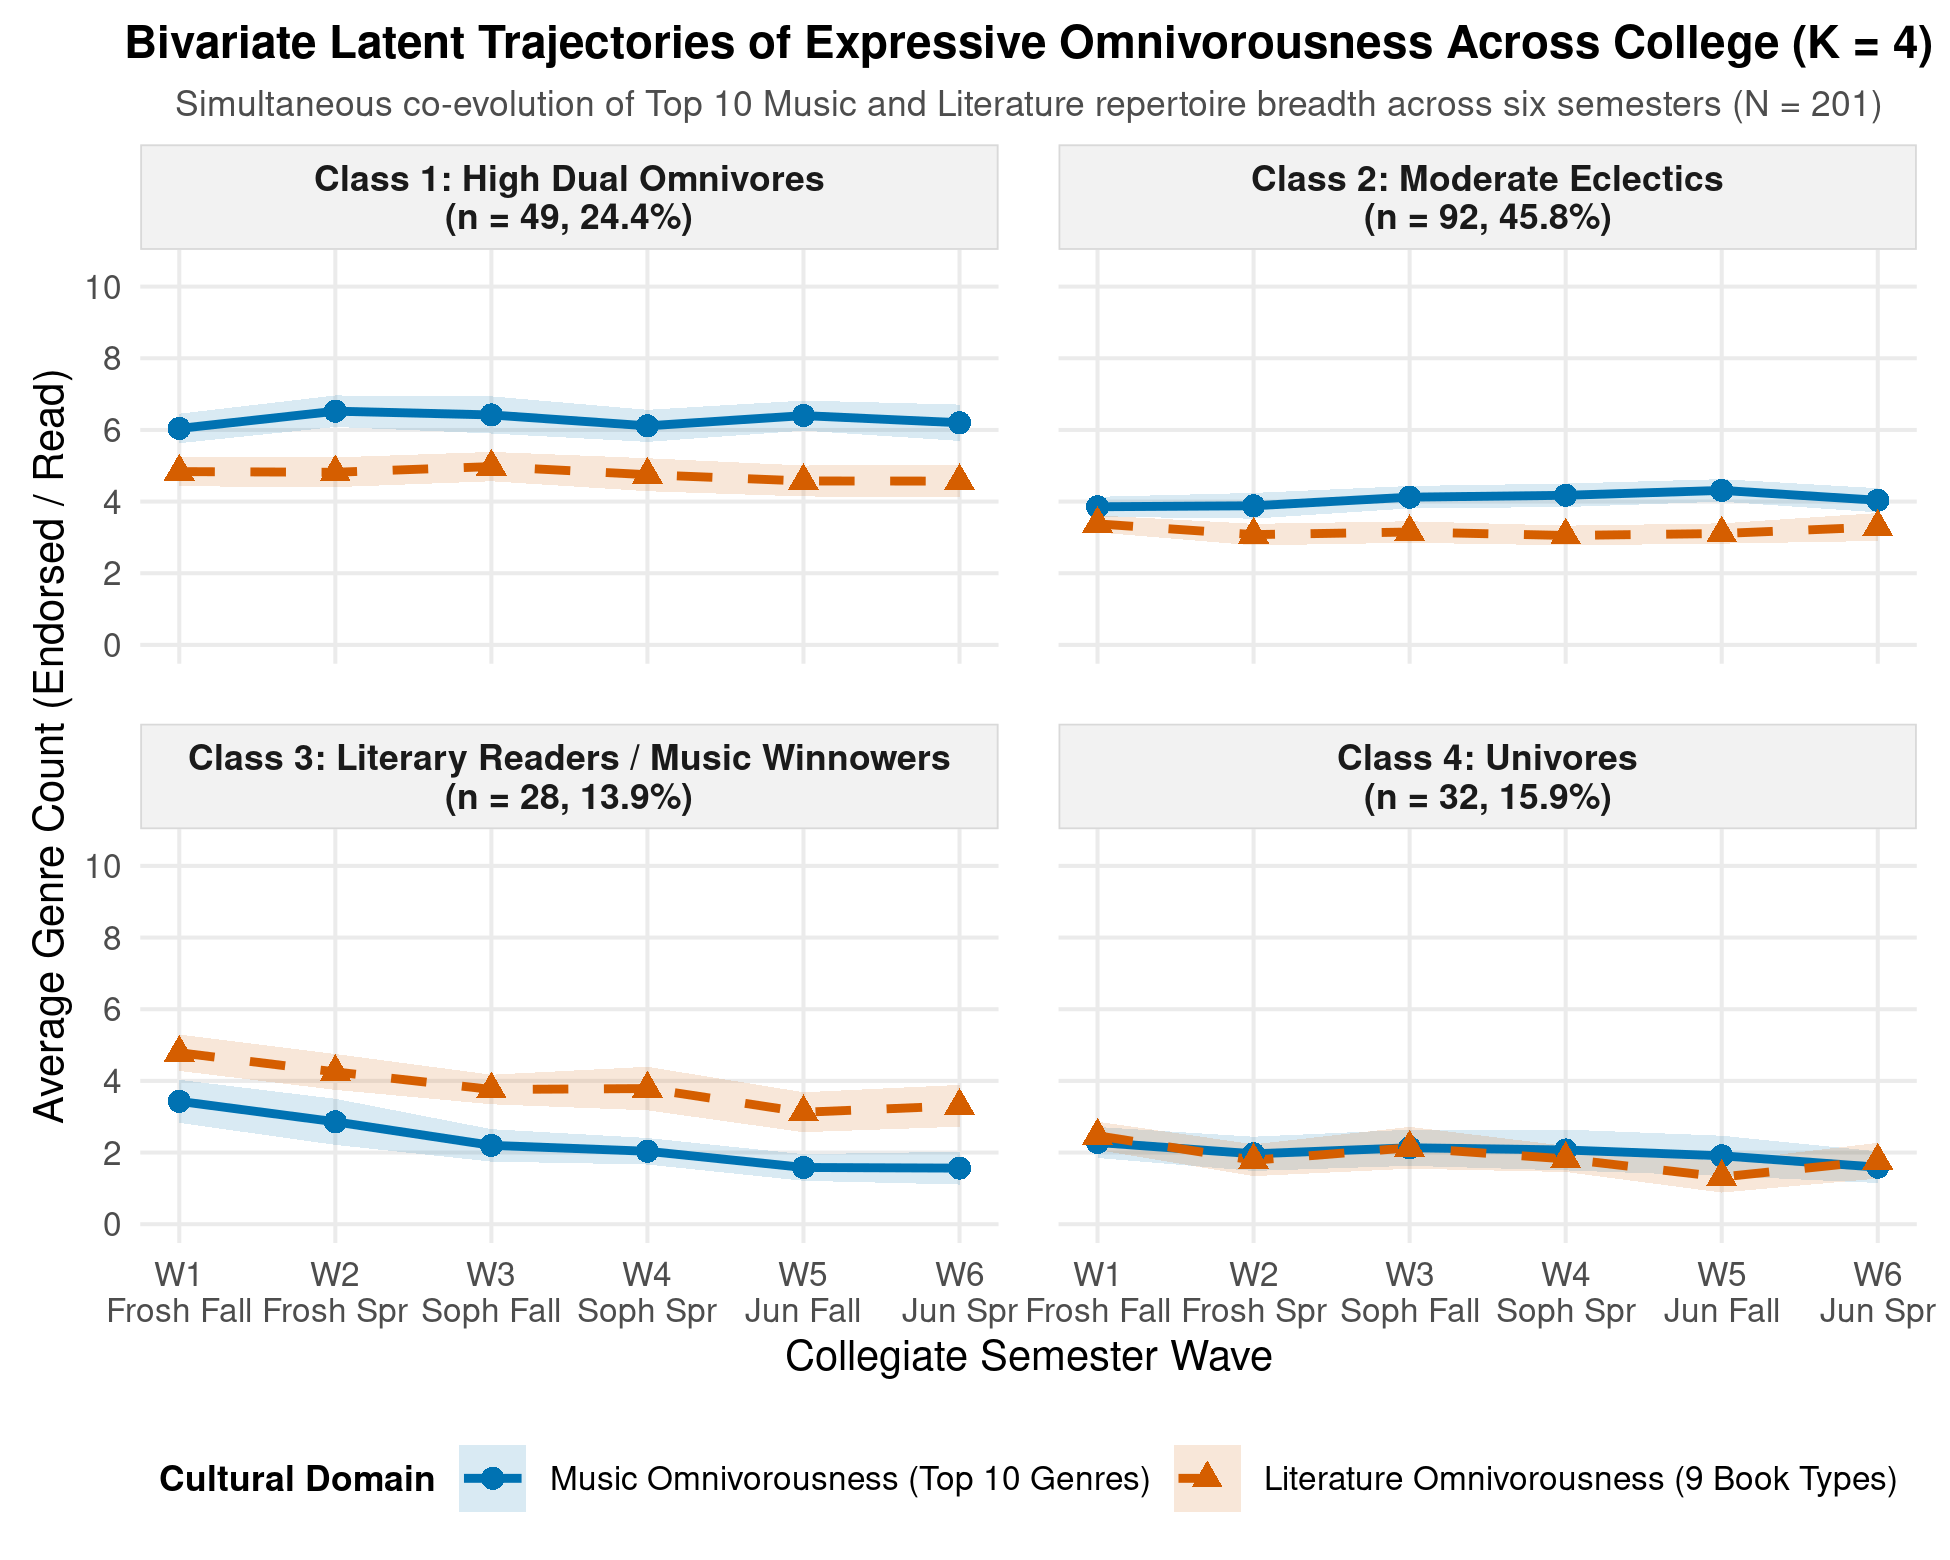
\includegraphics[width=\linewidth]{Plots/fig6_bivariate_omnivorousness_trajectories.png}
\caption{Bivariate latent trajectories of cultural omnivorousness across college from the 4-class Poisson growth mixture model (Waves 1 to 6, $N = 201$). Blue solid curves and circular markers denote Musical Omnivorousness (total genre count endorsed out of the Top 10 genres); orange dashed curves and triangular markers denote Literature Omnivorousness (total book genres read for leisure out of 9 items). Shaded ribbons indicate 95\% confidence intervals around empirical wave means.}
\label{fig:bivariate}
\end{figure}

The trajectory morphology in Figure~\ref{fig:bivariate} reveals four distinct patterns of cultural repertoire management:

First, ``Class 1: High Dual Omnivores'' ($n = 49, 24.4\%$) displays high cultural volume across both spheres throughout college. In music, their repertoire breadth begins at an average of 6.04 genres in freshman fall, expands to 6.52 genres by freshman spring, and remains sustained between 6.11 and 6.40 genres across all subsequent semesters. In leisure reading, they maintain an average of 4.57 to 4.98 book genres across all waves. These students embody dual cultural omnivorousness, actively cultivating broad, diverse repertoires in both auditory and literary media.

Second, ``Class 2: Moderate Eclectics'' ($n = 92, 45.8\%$) represents the modal undergraduate pathway. These students maintain a stable, moderate breadth across college, consistently endorsing between 3.86 and 4.31 musical genres and reading between 3.05 and 3.38 book categories across all six semesters. Their trajectories exhibit minimal fluctuation over time, showing neither expansive aesthetic broadening nor winnowing.

Third, ``Class 3: Literary Readers / Music Winnowers'' ($n = 28, 13.9\%$) exhibits a pronounced domain-asymmetric developmental profile. These students enter college with elevated leisure reading habits (averaging 4.79 book genres, on par with High Dual Omnivores) and maintain above-average reading engagement throughout college (3.12 to 4.25 genres). However, their musical preferences undergo a steep collapse: starting at a moderate 3.43 musical genres in freshman fall, their music repertoire plummets by 54.4\% down to 1.57 genres by senior year. Rather than withdrawing from cultural participation entirely, these students selectively abandon musical variety while remaining dedicated book readers.

Fourth, ``Class 4: Univores'' ($n = 32, 15.9\%$) enters college with modest repertoires (averaging 2.28 musical genres and 2.47 book genres) and undergoes progressive cultural winnowing across emerging adulthood. By senior year, their musical breadth contracts to 1.59 genres, while their leisure reading contracts to 1.32--1.77 genres. These students narrow their cultural engagement across both domains as collegiate academic demands accumulate.

\section{Predicting Pathway Sorting}

Panel B of Table~\ref{tab:bivariate} evaluates the predictive power of theoretical variable blocks in sorting students into these four bivariate pathways. Pre-collegiate scholastic capital (High School GPA and advanced degree aspirations) emerges as the primary sorting engine ($\chi^2 = 21.76, df = 6, p = 0.001$), significantly lowering AIC from 7759.7 to 7750.0. Collegiate context is marginally significant ($\chi^2 = 12.43, df = 6, p = 0.053$), reflecting the sorting influence of academic major. In contrast, family socioeconomic status (parental income and education) is completely non-significant ($\chi^2 = 1.89, df = 6, p = 0.930$). When all covariates are entered simultaneously, the full multivariable model achieves decisive statistical significance ($\chi^2 = 49.70, df = 27, p = 0.005$).

As detailed in Table~\ref{tab:app_coefs_biv}, multivariable parameter estimates indicate that entering college with high school academic achievement (mostly A/A- grades) acts as a primary protective barrier against cultural winnowing. Students with high prior GPA are over 85\% less likely to sort into Literary Readers / Music Winnowers ($\text{OR} = 0.121, p = 0.002$) and Univores ($\text{OR} = 0.134, p = 0.002$), while also being significantly less likely to enter Moderate Eclectics ($\text{OR} = 0.288, p = 0.037$) relative to High Dual Omnivores. Inverted, high scholastic capital increases the odds of sorting into the High Dual Omnivore trajectory by over eight-fold relative to Literary Winnowers ($\text{OR} = 8.26, p = 0.002$) and Univores ($\text{OR} = 7.46, p = 0.002$), and by 3.5-fold ($\text{OR} = 3.47, p = 0.037$) relative to Moderate Eclectics. 

Roman Catholic religious affiliation also significantly reduces sorting into all three non-omnivorous pathways ($\text{OR} = 0.224\text{--}0.321, p < 0.05$). Furthermore, academic major helps explain the domain asymmetry of Class 3: over 71\% of Literary Readers / Music Winnowers are non-STEM majors ($\text{OR} = 0.513$ for STEM), indicating that humanities and social science fields foster persistent literary reading despite the contraction of musical repertoires. Finally, the statistical null effect of parental income and education persists in the four-class count model, reinforcing the qualification that upstream institutional admissions filters at selective universities compress family socioeconomic variance, leaving prior scholastic achievement and campus context as the primary observable sorting mechanisms.

\begin{table}[htbp]
\centering
\small
\setlength{\tabcolsep}{4pt}
\caption{Multinomial Logistic Parameter Estimates and Odds Ratios from the Four-Class Bivariate Cultural Omnivorousness Model ($N = 201$)}
\label{tab:app_coefs_biv}
\begin{tabular*}{\linewidth}{@{\extracolsep{\fill}}lcccccc@{}}
\toprule
Predictor Variable & \multicolumn{2}{c}{\textbf{Class 2: Eclectics}} & \multicolumn{2}{c}{\textbf{Class 3: Lit Winnowers}} & \multicolumn{2}{c}{\textbf{Class 4: Univores}} \\
\cmidrule(lr){2-3} \cmidrule(lr){4-5} \cmidrule(lr){6-7}
& \textbf{Est (SE)} & \textbf{OR} & \textbf{Est (SE)} & \textbf{OR} & \textbf{Est (SE)} & \textbf{OR} \\
\midrule
Constant & 2.74 (2.65) & 15.52 & 3.51 (3.41) & 33.32 & 1.28 (3.59) & 3.60 \\
Woman (ref: Man) & -1.00* (0.40) & 0.37 & -0.58 (0.53) & 0.56 & -0.90 (0.53) & 0.41 \\
White (ref: Non-White) & -0.41 (0.54) & 0.66 & -0.20 (0.70) & 0.82 & -0.64 (0.68) & 0.53 \\
Catholic (ref: Non-Catholic) & -1.14* (0.50) & 0.32 & -1.29* (0.62) & 0.28 & -1.50* (0.61) & 0.22 \\
Parent Income (\$1,000s) & 0.01 (0.00) & 1.01 & 0.00 (0.00) & 1.00 & 0.01 (0.00) & 1.01 \\
Parent Education (Years) & -0.01 (0.12) & 0.99 & -0.07 (0.15) & 0.93 & 0.02 (0.15) & 1.02 \\
High School GPA (A/A-) & -1.24* (0.60) & 0.29 & -2.11** (0.67) & 0.12 & -2.01** (0.66) & 0.13 \\
Aspires to Advanced Degree & -0.55 (0.75) & 0.58 & -0.85 (0.92) & 0.43 & -1.40 (0.85) & 0.25 \\
STEM Major (ref: Non-STEM) & 0.14 (0.39) & 1.15 & -0.67 (0.55) & 0.51 & 0.13 (0.51) & 1.14 \\
Hometown Urbanicity & 0.10 (0.26) & 1.10 & 0.14 (0.32) & 1.15 & 0.36 (0.38) & 1.44 \\
\bottomrule
\end{tabular*}
\begin{minipage}{\linewidth}
\vspace{4pt}
\footnotesize
\textit{Note:} Estimates ($\beta$), standard errors in parentheses, and Odds Ratios ($\text{OR} = \exp(\beta)$) from the full multivariable endogenous multinomial logit model (\texttt{FLXPmultinom}) estimated jointly with the four-class bivariate Poisson growth model in \texttt{flexmix}. Reference category is Class 1: High Dual Omnivores ($n = 49$). * $p < 0.05$, ** $p < 0.01$, *** $p < 0.001$.
\end{minipage}
\end{table}

\bibliographystyle{apalike}
\bibliography{references}

\end{document}
